\documentclass[12pt, a4paper]{article}

\usepackage{amsmath}
\usepackage{array}
\usepackage{amsmath}
\usepackage[portuguese]{babel}
\usepackage{chngpage}
\usepackage{float}
\usepackage[a4paper, margin=2cm]{geometry}
\usepackage{graphicx}
\usepackage{hyperref}
\usepackage{listings}
\usepackage{setspace}
\usepackage{xcolor}

\lstdefinestyle{codestyle}{
    commentstyle=\color{teal},
    keywordstyle=\color{blue},
    numberstyle=\ttfamily\color{gray},
    stringstyle=\color{red},
    basicstyle=\ttfamily\footnotesize,
    breakatwhitespace=false,
    breaklines=false,
    keepspaces=true,
    numbers=none,
    showspaces=false,
    showstringspaces=false,
    showtabs=false,
    tabsize=4
}
\lstset{style=codestyle}

\title{\Huge \textbf{Computação Gráfica \\ \Large Trabalho Prático -- Fase II}}
\date{30 de março 2025}
\author{Grupo 3}

\begin{document}

\begin{center}
    
\includegraphics[width=0.25\textwidth]{res/cover/EE-C.eps}
\end{center}

\chardef\_=`_
\onehalfspacing
\setlength{\parskip}{\baselineskip}
\setlength{\parindent}{0pt}
\def\arraystretch{1.5}

{\let\newpage\relax\maketitle}
\maketitle
\thispagestyle{empty}

\vspace*{\fill}

\begin{adjustwidth}{-2cm}{-2cm} % These values only need to be large enough to center the table
    \begin{center}
        \begin{tabular}{>{\centering}p{0.25\textwidth}
                        >{\centering}p{0.25\textwidth}
                        >{\centering}p{0.25\textwidth}
                        >{\centering\arraybackslash}p{0.25\textwidth}}
            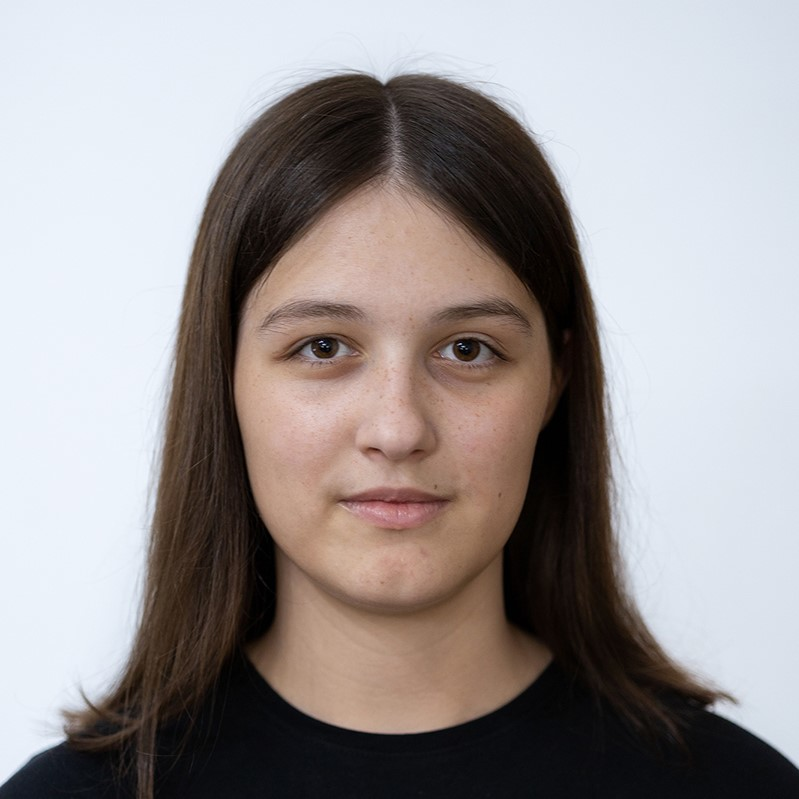
\includegraphics[width=3.5cm]{res/cover/A104437.png} &
            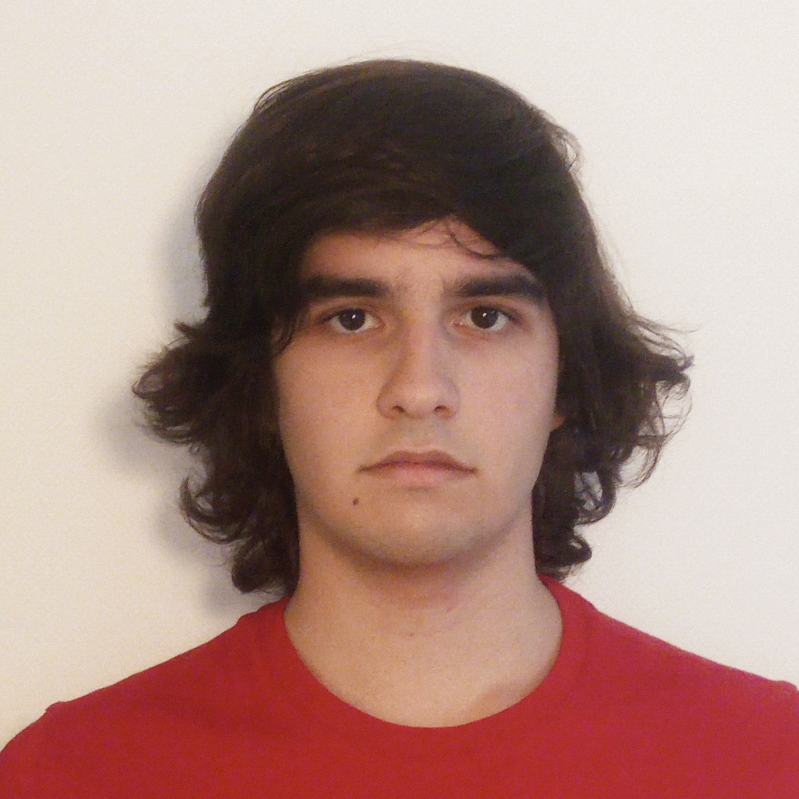
\includegraphics[width=3.5cm]{res/cover/A104348.png} &
            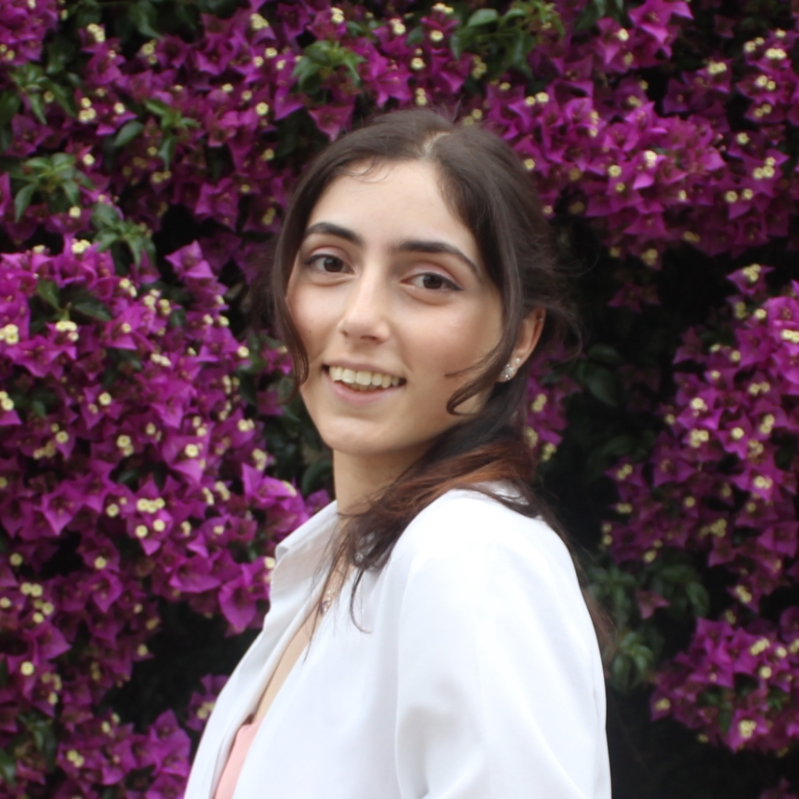
\includegraphics[width=3.5cm]{res/cover/A90817.png} &
            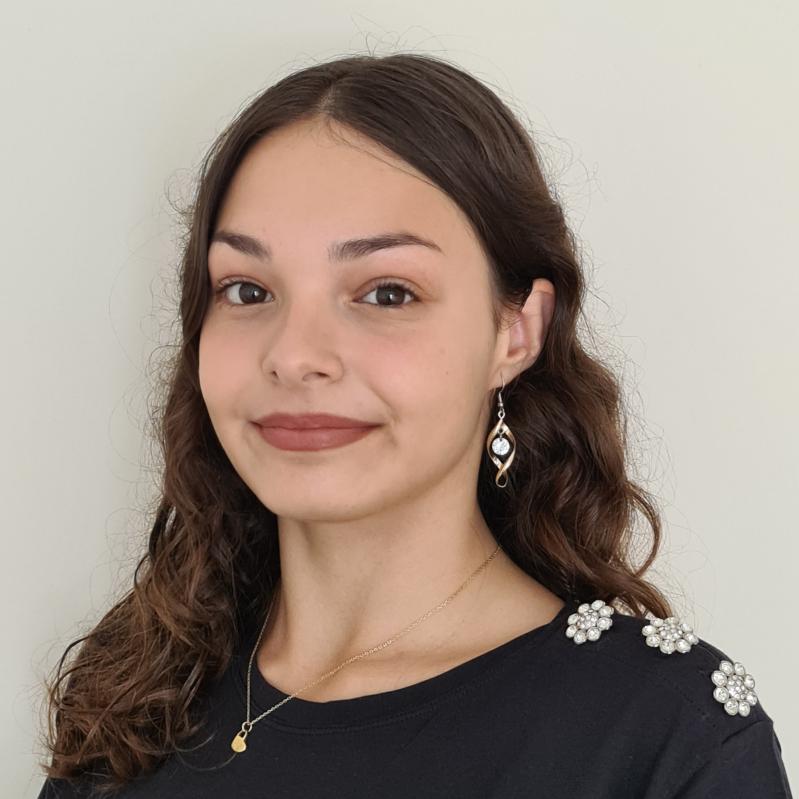
\includegraphics[width=3.5cm]{res/cover/A104179.png} \\

            Ana Oliveira & Humberto Gomes & Mariana Cristino & Sara Lopes \\
            A104437      & A104348        & A90817           & A104179
        \end{tabular}
    \end{center}
\end{adjustwidth}

\pagebreak

\begin{abstract}
    \textbf{\color{red} TODO - resumo}
\end{abstract}

\section{Generator}

\subsection{Câmara Livre}

EM FALTA INTRODUÇÃO

\subsubsection{Movimentação}

A câmara livre permite que o utilizador se desloque de forma intuitiva, sendo esta semelhante à
de jogos de exploração na primeira pessoa, como simuladores de voo, e aplicações interativas 3D,
como ambientes de realidade virtual. Para isto, são realizadas translações em diferentes eixos e
a orientação da câmara é alterada através de rotações. De seguida, descrevem-se os diferentes tipos
de movimento suportados:

\begin{itemize}
    \item \textbf{Translação horizontal:} A câmara pode mover-se para a frente e para trás ao longo
    do vetor \emph{front}, e para os lados ao longo do vetor \emph{right}.
    \item \textbf{Translação vertical:} O movimento vertical ocorre ao longo do vetor \emph{up},
    permitindo ao utilizador subir e descer livremente.
    \item \textbf{Rotação:} A orientação da câmara muda com base nos valores de \emph{yaw}
    (rotação horizontal) e \emph{pitch} (inclinação vertical), o que permite alterar a direção do
    olhar.
\end{itemize}

A posição da câmara é atualizada da seguinte forma:

\[
\text{posição} \gets \text{posição} + \text{velocidade} \times \text{direção}
\]

onde o vetor que representa a direção depende do movimento escolhido pelo utilizador. Ou seja, a
direção correponde ao vetor \emph{front}, \emph{right} ou \emph{up}. A rotação, controlada pelo
\emph{pitch} e pelo \emph{raw}, afeta o vetor \emph{front} diretamente. Sempre que a orientação da
câmara muda, os vetores \emph{right} e \emph{up} são recalculados para que os movimentos laterais
continuem de acordo com a perspetiva atual da câmara.

\section{Transformações}

\textbf{\color{red} TODO - transformações}

\section{Modelo estático do sistema solar}

\textbf{\color{red} TODO - sistema solar}

\section{Extras}

\textbf{\color{red} TODO - extras}

\section{Resultados obtidos}

\textbf{\color{red} TODO - resultados}

\section{Conclusão e Trabalho Futuro}

\textbf{\color{red} TODO - conclusão}

\begingroup
\section{Bibliografia}
\renewcommand{\section}[2]{}

\begin{thebibliography}{9}
    \bibitem{exemplo}
        \href{https://youtu.be/dQw4w9WgXcQ}{Um item de exemplo na bibliografia}
\end{thebibliography}
\endgroup

\end{document}
